%===================================================================================================
%  Chapter : 力学の基本概念
%  説明    : 力,重ね合わせの原理,力(作用)の種類,単位などの基礎概念について説明する.
%===================================================================================================
%   %==========================================================================
%   %  Section
%   %==========================================================================
    \section{力とその性質}
%       %======================================================================
%       %  SubSection
%       %======================================================================
        \subsection{力(ちから)}
            世の中には,\textbf{力} といわれる現象がある.この「力」は様々な意味
            合いで使用される.視力,脚力,握力などの身体能力に関する「力」.計算
            力,想像力などの思考に関する「力」.ほかにも,技術力,接客力,情報収
            集力,対応力など,人の性格や能力に関する「力」などいろいろ考えられる.

            物理学で対象とする \textbf{力} は,弾性力や反発力,物体を変形させる力,
            物体の運動方向を変化させる力などである.以下,「力」と表現される場合
            には,特に断りのない限り,このような力を想定する.

            力とは,捕らえ所がなく,非常に曖昧である.現に,ニュートン力学では,
            力とは何かを説明することはできない.では,どのように力というものを
            考えるのか.結論から言うと,力の存在を,なんの根拠もなしに認めること
            である.力という物理現象の発生原因が分からないのだけど,実際に,
            私たちは日常的に,力が存在しているということに関して,疑いを持つこと
            はない
                \footnote{
                    力の存在に疑問をもつこともあることだろう.しかし,ここ
                    では哲学について語っているのではない.力とは何か,も
                    っと言うと,力という現象を感じる私たちとは何なのか,こ
                    れはひどく難しい問題である.なので,こういう問題には目
                    を閉じておくことにしよう.今の私の興味は,世界がどのよ
                    うに構成されているかということであり,こんなところで,
                    足を止めてしまってはならない.知りたいことはもっと先に
                    ある.そのために,力という現象の存在を素直に認めること
                    にしよう.ただし,この問題を忘れてはならない.ノートの
                    端の方に,「力とは何か」という疑問をメモしておこう.
                }.

            しかしながら,力は重要な概念である.
            力学の最大の目標の一つは,物体の運動の軌道を求めることにある.
            それには,物体にかかっている力を,考えないとならない.
            物体の運動の原因は力であり,力は
            物体の運動を解析する上で,非常に重要なものである.

            これだけ重要な概念である“力”なのだけど,「力とは何か」と問われると,
            回答するにはとてもむづかしい
                \footnote{
                    素粒子物理学の教科書などでは,(ゲージ粒子を介した)「相互作用」と
                    説明されるが,詳細は,素粒子物理を考えるときに説明しよう.
                }.
            とりあえずの力の説明として,物体を変形させる,あるいは,物体の位置を
            変化させる原因としておこう.言い換えると,物体が変形すれば,その物体に
            力が加えられたということになるし,物体の位置が変化したならば,この場合にも
            物体に力が加えられたということになる.

            物体の変形や変位を説明する概念として,力の存在が要請されるとしてもよい.

%       %======================================================================
%       %  SubSection
%       %======================================================================
        \subsection{力の重ね合わせの原理}
            複数の力が物体に働いているとき,その力を合計することを,
            力の \textbf{合成} という.合成された力のことを \textbf{合力} という.
            力の合成は,ベクトル和 で表現できる.すなわち,物体に $N$ 個の力が加わっているとき,
            その合力は,
                \begin{align}
                    \bF_{\mbox{合力}}
                    = \bF_{1}+\bF_{2}+ \cdots + \bF_{N}
                \end{align}
            である.和の記号を用いると
                \begin{align}\label{gouryouku_gouryoku}
                    \bF_{\mbox{合力}} = \sum^{N}_{i=1} \bF_{i}
                \end{align}
            のようにかける.

            また,逆に,1つの力を,複数の力の合力である
                \footnote{
                    式(\ref{gouryouku_gouryoku})は等式であり,
                    左右が等しいのだから明らかではあるが,
                    少しだけ気付きにくいかと思われたので書いておいた.
                    すなわち,1つの力を複数の力に \textbf{分解} することもできる.
                    }.
            力の分解は,よく行われる.例えば,$x-y$ 平面上における力を表現するのに,
            力を $x$ 方向と $y$ 方向に分けて考えることが多い.
                \begin{figure}[hbt]
                    \begin{center}
                        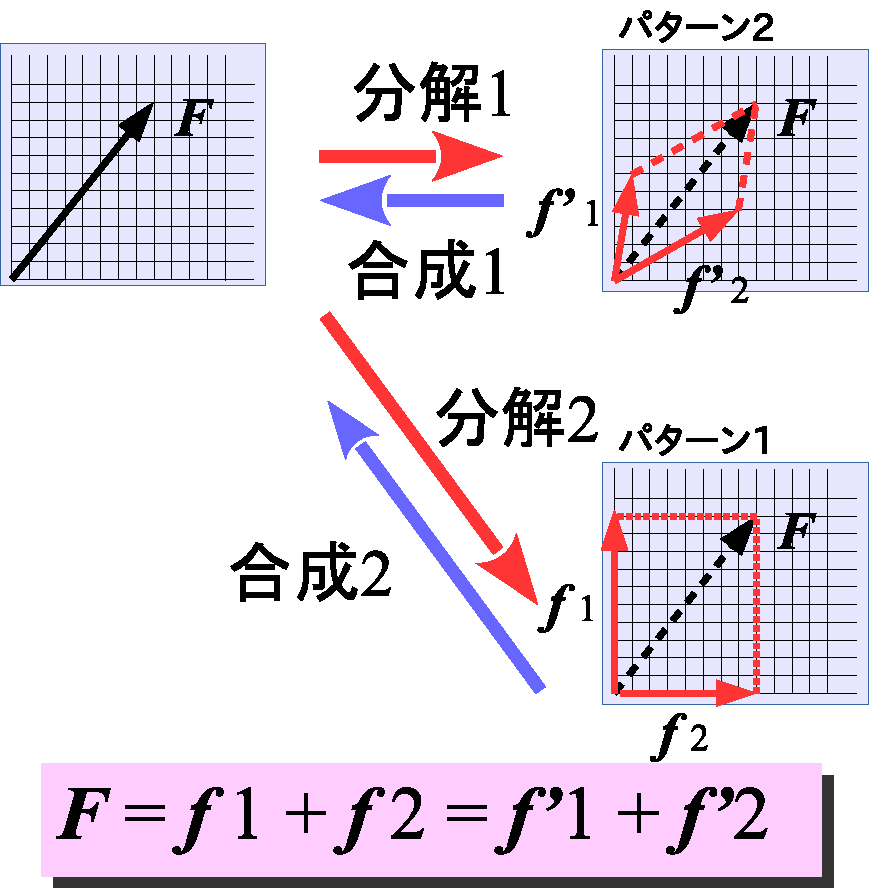
\includegraphics[keepaspectratio, width=6cm,height=6cm,clip]{f_bunkai.pdf}
                        \caption{力の合成,力の分解}
                        \label{fig:f_bunkai}
                    \end{center}
                \end{figure}

            力学では,力が重ね合わせの原理を満たす理由は問わない.
            この原理は,実験的に確かめられる法則として扱われている
                \footnote{
                    もしかしたら,将来,このことを説明できる日が来るかもしれないが,
                    今はこれを説明できるだけの知識がない.ただ,電磁気力に関していえば,
                    電磁場の線形性に帰着できる(問題を先送りしただけ,かもしれないが).
                }.

            別称として,\textbf{平行四辺形の法則},\textbf{力学の第0法則} とかと表現されることもある.
            重ね合わせの原理が成り立つことを,数学的に表現すると,「力には \textbf{線形性} がある」ともいえる.
            もっと物理学の学習を続けていけば,力の重ね合わせの原理を
            説明できるようになるのかもしれない.しかし,ここではその理由はわからないので.
            とりあえず,重ね合わせの原理を認め,学習を先に進めるべきだ.

              \begin{memo}{和の記号: $\sum$}
                例えば任意の4つの実数 $a_{0},\,a_{1},\,a_{2},\,a_{3}$ が与えられたとする.
                この時,$a_{0}$ から $a_{3}$ までの和 $S$ を書き表すとき,
                  \[
                    S = a_{0} + a_{1} + a_{2} + a_{3}
                  \]
                のように書き表せる.しかし,項数が9999個になった場合($a_{1},\,a_{2},\,\cdots\,a_{9999}$ ),
                書き表すことはできない
                  \footnote{
                    原理的には可能であるが,実際に書くのに時間がかかるため現実的ではない.
                  }.
                そこで,$a_{0}$ から $a_{9999}$ までの数の合計を計算することを示す記号を導入したくなる.
                和の記号として,$\sum$ を新たに導入し,以下のように記述することにしよう.
                  \[
                    \sum^{9999}_{i=0} a_{i} := a_{0} + a_{1} + a_{2} + \cdots + a_{9999}.
                  \]
                $\sum$ は「シグマ(Sigma)」と発音する.
                今の例だと上限が9999の場合に限ってしまうが,上限を任意の数 $N$ として場合には,
                次にように書く
                  \footnote{
                    前の例だと具体的な数字だった9999を $N$ という文字に変更する.
                  }.
                  \[
                    \sum^{N}_{i=0} a_{i} := a_{0} + a_{1} + a_{2} + \cdots + a_{N}.
                  \]
                さらに,この例だと最初の数字は0であるが,もちろん任意でよい.
                最初の数を $m$ と文字で置き換えて($m<N$であるはず),
                  \footnote{
                    例えば,$a_{0},\,a_{1}$ がべっと定まっていて,この2つの数にさらに
                    $a_{2}$ から $a_{N}$ までの数の合計を足したいこともありうる.
                  }
                  \[
                    \sum^{N}_{i=m} a_{i} := a_{m} + a_{m+1} + a_{m+2} + \cdots + a_{N}.
                  \]
                  これで,項数が多くなっても和を書き表せるようになった.

                  ちなみに,$a_{i}$ の添え字 $i$ は和の具体的な計算(和の記号の展開)の時に,
                  失われてしまう数で\textbf{ダミー}の数字と言われることがある.別に $i$ ではなく,
                  $j$ を使ってもよい.
                  その場合は以下のようになるが,$i$ の場合と意味は同じである.
                  \[
                    \sum^{N}_{j=m} a_{j} := a_{m} + a_{m+1} + a_{m+2} + \cdots + a_{N}.
                  \]

                  項数を無限大 $\infty$ にした場合でも,
                  \[
                    \sum^{\infty}_{j=m} a_{j} := a_{m} + a_{m+1} + a_{m+2} + \cdots
                  \]
                  と形式的に表現することもできる
                    \footnote{
                      「形式的に」といったのは,$\infty$ が数ではないために,正式な和の手続きに
                      なっていないからである.しかし,この表現により,無限にある項数を順に足し合わせる
                      という行為をイメージさせることが可能である.
                    }.
              \end{memo}


%       %======================================================================
%       %  SubSection
%       %======================================================================
        \subsection{作用}
            力のことを,場合によっては,\textbf{作用} ということもある.
            例えば,「2つの物体間に働く相互作用」と書かれていたら,
            これは,2つの物体に働く力という意味である
                \footnote{
                    量子力学や素粒子理論,あるいは,一般相対性理論の教科書でよく使われる表現だ.
                    ニュートン力学でも,「作用$\cdot$反作用の法則」のように使用されれる.
                }.

            宇宙論や素粒子理論の教科書などでは,その冒頭に「力には4つの種類ある」
            と紹介さることが多く,\Table\ref{table:f4force} が掲げられる
                \footnote{
                    当然ながら,この力の分類は,物理学の発展により得られたものであり,
                    最初から知られていた事実ではない.
                }
            この4つの力は,それそれで従っている物理法則や性質が異なる.
            つまり,少なくとも4つの物理法則があるということであり,
            だけどこれは,物理法則はただひとつであるという物理学の精神に反する.
            物理学の理論構築の目標の一つは,この4つの力を自然に説明することである.
            要するに,4つの力を説明できるような,もっと大きな理論的枠組みを構成し,
            その枠組みの中で4つの力が自然に導かれるような理論を作りたいのだ
                \footnote{
                    今では,電磁気力と弱い相互作用と強い相互作用の3つの力を説明できる
                    統一理論が知られいて,これを \textbf{標準模型} という.しかし,
                    標準模型には人為的な定数が多く含まれており,また,万有引力も
                    説明できないので,私達が知りたい力の統一理論ではない.

                    当然ながら,力を統一的に説明できるという保証はどこにもない.
                    統一理論の確立は可能であると信じて,理論を作り上げる努力をするしかない.
                    超弦理論は,現状での最も有力な理論の1つであるが,超弦理論を実験的に検証されていない.
                    他の候補にもループ量子重力という理論も提案されているが,こちらも実験検証ができていない.
                    一般に周知される理論の確立にはまだ時間がかかるようだ.
                    もしかしたら,その過程で,力を統一的に説明できない,という結論に至る可能性もある.

                }.

                 \begin{table}[htb]
                  \centering
                  \caption{4種類の力}
                  \begin{tabular}{|l|c|}           \hline
                    名称         & 別称         \\ \hline  \hline
                    万有引力     & 重力         \\ \hline
                    電磁気力     & ローレンツ力 \\ \hline
                    弱い相互作用 & $\beta$崩壊  \\ \hline
                    強い相互作用 & 核力         \\ \hline
                  \end{tabular}
                  \label{table:f4force}
                \end{table}

            \begin{mysmallsec}{万有引力(重力)}
            万有引力はどんな物質も持っている性質で,その強さは,4つの内で最弱.
            重力とはが物を引っ張る力のことで,それは万有引力の一部であるが,
            重力という表現のほうが実感があり馴染み易いせいか,万有引力と同義的に
            使われることが多い.一般的に,万有引力と重力は同義であると考えてよい
                \footnote{
                    ただし,両者を区別して考えたい場合もあるので,文脈により判断したい.
                }.

            重力を説明する理論は一般相対性理論である.重力があまり強くない場合は,
            ニュートンの力学で十分精度よく説明される.
            \end{mysmallsec}

            \begin{mysmallsec}{電磁気力(ローレンツ力)}
            電磁気力は,ローレンツ力と言われることもある.ローレンツは電磁気現象の
            解明に貢献した物理学者の名前である.電磁場中を運動する電荷が受ける力の
            ことである
                \footnote{
                    詳しくは電磁気学の部分で学習する.
                }.

                        電磁気力は電磁気学,あるいは,電弱統一理論によって説明される.
                        電弱統一理論は電磁気力と次に説明する弱い相互作用の両方を説明できる理論である.
                        ただ,電磁気力のみを考える際には,マクスウェルの古典的な電磁気学
                        で十分な場合が大半.
            \end{mysmallsec}

            \begin{mysmallsec}{弱い相互作用}
            弱い相互作用とは,原子が$\beta$崩壊するときに使われる力である.原子核や
            素粒子を扱う場合に,重要な力だけれど,力学では対象範囲外の概念である.
            量子力学や特殊相対性理論(場の理論)によって説明される力である.
                        電弱統一理論によって説明される.
            \end{mysmallsec}

            \begin{mysmallsec}{強い相互作用(核力)}
            強い相互作用とは,原子核を構成する陽子と中性子を結びつける力である.
            陽子と陽子,中性子と中性子も強い相互作用によって引き合っている.
            電磁気力を考えると陽子同士は反発しあって安定しないのだが,この
            強い相互作用によって引き合うために,原子核が安定して存在できる
            だから,当然,強い相互作用は電磁気力よりも強い力である.しかし,
            単純にそう考えると,電磁気力は強い相互作用に隠されてしまう(
            表だって電磁気力を感じなくなってしまう)はずだが,実際はそうではない.
            その理由は,有効範囲の違いで説明される.原子核よりも狭い領域では
            強い相互作用が優勢であるが,原子核以上の範囲では強い相互作用は
            電磁気力よりも弱くなるのだ.
                        各力は,量子色力学によって説明される.
            \end{mysmallsec}

%       %======================================================================
%       %  SubSection
%       %======================================================================
        \subsection{外力}
            系の外から生じる力が系に影響を及ぼすこともあろう.対象とするもの以外
            から受ける力のことを \textbf{外力} という.例えば,重力に
            逆らって物体を持ち上げるときに,人間による力が必要である.物体が勝手
            に重力に逆らって宙に浮いたりすることはありえないからである.このよう
            に,人間による力を想定して,外力という言葉を使うこともある.

%   %==========================================================================
%   %  Section
%   %==========================================================================
    \section{基本単位 ([s]/[m]/[kg]/[A])}
%       %======================================================================
%       %  SubSection
%       %======================================================================
        \subsection{単位と測定}
            物理学は経験・実験結果がその基礎であることは前に書いた通りである.
            実験とは,実験すべき対象に何か刺激を与えて,その反応をみることである.
            このとき,対象の持っている何らかの量を測る必要が出てくる.ここで,「
            「測定とは何か」ということを考え直さないといけない.
            答えは簡単だ.
            \textbf{測定とは,基準値に対して何倍であるかを調べる行為である}と言える.
            言い方を変えれば,測定基準と測定対象の大きさを比較することである.
            測定対象は色々とあるが,例えば,音の大きさだったり,気圧,
            紐の長さ,ものの色,糖度,$\cdots$ etc,と色々ある.
            この比較対象となる基準値は,\textbf{単位} と呼ばれる.
            「基準値」という語彙は意味が広く,合格基準点とかのボーダーライン的な
            意味でつかわれることも多い.単位という特別な名称を与えたのは,基準値
            の意味を狭めるためである.単位とは,測定対象の大きさや量を数字で示す
            ための,最も基本的な大きさを規定するものである.

        \subsection{4つの基本単位}
            物理学では,以下の4つを,測定可能な最も基本的な量としている(\Table\ref{table:f4unit})
            \footnote{
                逆に言うと,この4つの単位は,他から導くことのできない単位である.
                いわば,単位系におけるもっとも素朴な要素となる.単位の素粒子的な
                役目を担っている.他の単位は,これらの単位から組み立てることが
                できる,というか,そのように定義される.
            }.
                \begin{table}[htb]
                  \centering
                  \caption{基本単位(物理学の基本4単位)}
                  \begin{tabular}{|l|c|c|l|}                  \hline
                    名称 & 記号   & 英字表記  & 読み       \\ \hline  \hline
                    時間 & [s]    & second    & セカンド   \\ \hline
                    長さ & [m]    & meter     & メートル   \\ \hline
                    質量 & [kg]   & kilo-gram & キログラム \\ \hline
                    電流 & [A]    & ampere    & アンペア   \\ \hline
                  \end{tabular}
                  \label{table:f4unit}
                \end{table}

            この4種類の単位が,現在の物理学の \textbf{基本単位} である.
            これらは,国際単位系であるSI基本単位に指定されている.
            ちなみに,SI単位系には,これら4つほかに,以下の3つが挙げられている(\Table\ref{table:o4unit}).
                \begin{table}[htb]
                  \centering
                  \caption{他の基本単位}
                  \begin{tabular}{|l|c|c|l|}                      \hline
                    名称       & 記号   & 英字表記 & 読み      \\ \hline \hline
                    熱力学温度 & [K]    & kelvin   & ケルビン  \\ \hline
                    物質量     & [mol]  & mol      & モル      \\ \hline
                    光度       & [cd]   & candela  & カンデラ  \\ \hline
                  \end{tabular}
                  \label{table:o4unit}
                \end{table}

            しかし,熱力学を考える場合の熱力学温度[K]を除き,
            物理学的観点からは,この3つは基本単位とは考えない.
            物質量の[mol]は化学における重要な単位であるが,
            これは,統計物理学から定義できる量である.
            また,光度[cd]は光の強さを表している.電磁気学により,
            光は電磁波であることが示されており,その強さは電磁波の
            波長(もしくは周波数)で表せる.さらに言うと,実は熱は現実には存在しない.
            熱は,統計物理学によって,多数の分子の乱雑な運動であると説明される.
            つまり,日常で感じている熱とは,分子集団の持つ運動エネルギーであると
            言い換えられる.なので,これらの3つの単位は,他から導くことが
            できるという点で,物理学の基本単位としては,扱われていない.
            もちろん,基本単位でないからと言って,無意味ということではない.
            現象を簡潔に説明できる場合には,この3つの単位も積極的に使用される.

%       %======================================================================
%       %  SubSection
%       %======================================================================
        \subsection{組立単位}
                その他の単位として,例えば,角度を表現する[rad]や,光の強さを表現する[cd]
                などがある.角度は長さと同じに扱えるが,実際のイメージに即して考える場合に,
                欠くことのできない単位である(非常に便利であるという意味で).

                また,力やエネルギーの単位は,基本単位で構成される \textbf{組立単位} である.
                例えば,力の単位は[N](「ニュートン」と読む)であり,これを基本単位に
                分解すると,
                \begin{equation*}
                    [\mbox{N}] = [\mbox{kg}\cdot\mbox{m}/\mbox{s}^{2}]
                \end{equation*}
                となる
                    \footnote{
                        日本語による読み方は,
                        「キログラム メートル 毎秒毎秒(まいびょうまいびょう)」である.
                    }.
                エネルギーの単位[J](「ジュール」と読む)は,
                \begin{equation*}
                    [\mbox{J}] = [\mbox{Nm}] = [\mbox{kg}\cdot\mbox{m}^{2}/\mbox{s}^{2}]
                \end{equation*}
                    \footnote{
                        日本語による読み方は,
                        「ニュートン メートル」である.
                        基本単位に戻ると,
                        「キログラム メートル二乗 毎秒毎秒(まいびょうまいびょう)」となる.
                    }.
                力やエネルギーの性質などについては,後で学習する.ここで覚えておくべきことは,
                後の学習で現れる全ての物理量は,4種類の基本単位から組み立てられているということ
                である.

%       %======================================================================
%       %  SubSection
%       %======================================================================
        \subsection{測定の方法}
            測定とは,測定対象の大きさを知るための行為である.物体が大きいとか,小さい
            とかという判断は,どのように行うべきだろうか.例えば,単に大きな
            消しゴムとか,小さい鉛筆とかと言ったところで,具体的な大きさを思い
            描くことは不可能である.確かに,これまでの経験から常識的な大きさを
            思い描いて,これと比較することで,大きいだとか小さいだとかというこ
            ともある.しかし,これは日常生活でのはなしであって,物理学において
            は,このような曖昧さは避けるべきだ.常識的な大きさと言われても,
            その思い描く大きさは人それぞれだし,ましてや常識的な大きさよりも大
            きいと表現されてしまっては,具体的な大きさは全く想像がつかない.

            では,物の大きさを具体的に,しかも誰にとっても同じような大きさが想
            像できるように表現するには,どうしたら良いだろうか.答えはもう出て
            しまっている.\textbf{単位} という概念を導入するのである.単位とい
            う概念を導入することで,物体の大きさを具体的に表現できる
            ようになるのだ.

            例えば,ここに2つの異なる長さの棒があるとしよう.簡単のため,この2
            つの棒はまっすぐであるとする.2つの棒は長さの違いで区別することがで
            きて,長い方をA,短い方をBとしよう.今,何も考えずに“長い方”ある
            いは“短い方”と書いてしまったが,どのように長さを測ったのだろうか.

%       %======================================================================
%       %  SubSection
%       %======================================================================
        \subsection{単位}
            \textbf{単位} とは,測定の基準のことである.物理学は,物体の長さ
            や重さ,時間,電流値を最も基本的であるとしている.そして,力学では,
            この内の三つ,すなわち,\textbf{時間}$\cdot$\textbf{長さ}$\cdot$\textbf{重さ}
            を特に重要視する.これらはすべて実験的に観測されるものである.単位
            の重要性について,より具体的に「大きい」という言葉を例に取り,以下
            に説明してみよう.


%       %======================================================================
%       %  SubSection
%       %======================================================================
        \subsection{時間}
            時間の進みは,あらゆる空間において,一定である.時間を $t$ で表す.
            時間の単位を [s] で表す.「second」 又は 「秒」 と読む.
            時間は 過去$\rightarrow$現在$\rightarrow$未来 と進むと考える
                \footnote{
                    ここで注意しておく.今までのところ,
                    未来$\rightarrow$現在$\rightarrow$過去という風に,
                    私達が実感している時間の向きとは
                    逆の向きに時間が進んでも,物理法則が矛盾するようなことはない.
                    但し,熱力学の第2法則(「エントロピー増大の法則」:$\leftarrow$後述)は,
                    この限りではない.
                }.
            \begin{myshadebox}{単位時間(1[s])の定義}
                「${}^{133}${\rm Cs} 原子が出す電磁波が 9192631770 回振動する時間」が1[s] と定義される.
                原子の振動回数を数えることで1秒を測るということである.
            \end{myshadebox}

            \begin{memo}{“時間”と“時刻”の違い}
                ここで,「時間」と「時刻」の違いを確認する.
                言葉よりも,図で示したほうが早い(図\ref{fig:jikoku-to-jikan}).
                \begin{figure}[hbt]
                    \begin{center}
                        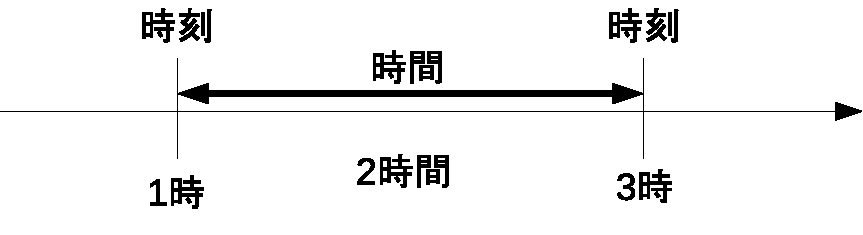
\includegraphics[keepaspectratio, width=7.2cm,height=3.6cm,clip]{jikoku-to-jikan.pdf}
                        \caption{時間と時刻}
                        \label{fig:jikoku-to-jikan}
                    \end{center}
                \end{figure}

                例えば,「1時から3時までの時間は2時間である.」という主張をするとき,
                この“2時間”が \textbf{時間} であり,1時とか3時は \textbf{時刻} である.
                時刻は幅がなく,時間を直線で表現にしたときには,点で表現される.
                それに対して,時間はある時刻と別の時刻の間の間隔である.

                勘違いを起こしがちなことがある.それは,
                すべての時刻を集めたものが時間である,という考えである.
                しかし,これは間違いだ.
                時間は数直線で表すことができ,よく,\textbf{時間軸} と
                いう言葉で表現される.時刻とは,時間軸の一点を表す語彙であるが,
                その一点には幅はない.つまり,時刻の時間は0である.0をいくらたくさん
                足しあわせたところで,結果は0であることは言うまでもない.
            \end{memo}

            \begin{memo}{飛ぶ矢のパラドクス}
                エレアのゼノン
                    \footnote{
                        $Z\eta \nu \omega \nu$(B.C.490 -- B.C.430, 古代ギリシア):
                        ギリシャ文字をそのままアルファベットに変換すると「Zhenon」.
                        しかし,英語表記で「Zeno」(ラテン語,フランス語でも同じ)で,
                        ドイツ語表記では「Zenon」と表される
                        (ドイツ語の場合,「ツェノン」と発音するのかな).
                        「エレアのゼノン」とも言われる.古代ギリシャ人.
                        ちなみに,「キプロスのゼノン」と呼ばれる,同名の人物がいるが,
                        その人とは別人.「エレアのゼノン」と書いたのも,それと区別するため.
                        キプロスのゼノンも,大哲学者であり,
                        ストア派と言われる禁欲的な態度や特を重んじる思想や態度を唱えた.
                    }
                は,次の4つのパラドクスを考えだしたことで,有名な人物である.
                    \begin{enumerate}
                        \item 二分割のパラドクス
                        \item アキレスと亀のパラドクス
                        \item 飛ぶ矢のパラドクス
                        \item 競技場のパラドクス
                    \end{enumerate}
                この内,3番目の「飛ぶ矢のパラドクス」が時間に関するパラドクスである.
                このパラドクスは,次のようなものである.動いている物体といえども,ある瞬間
                には,定まった1つの位置に位置しているはずである(写真をとるとその一点に位置している).
                定まった位置に存在するということは,静止しているのと同じ.ということは,
                動いうている物体は,瞬間的には静止しているということなる.つまり,動いている物体は,
                すべての瞬間で静止状態にあるということになる.明らかに,矛盾だ.この矛盾を
                「飛ぶ矢のパラドクス」という.
            \end{memo}

            \begin{memo}{時間とは何か}
                時間とは,一体,どこから生じているのか.
                いや,言い方を変えよう.なぜ私には時間という感覚があるのか.
                人間の知覚は五つあり,五感といわれる.
                それは,視覚,聴覚,嗅覚,触覚,味覚
                であるが,どれも直接的に時間を感じ取る器官ではない.
                それもそのはずで,「時間」という概念は外から与えられるもの
                ではなく,頭の中で作られるものだからだ.物の変化を感じ取るとき,
                頭の中で時間という感覚が生まれるのだ.

                自動車が走っているのを見て(視覚),時間を感じる.
                音楽を聴いているとき(聴覚),時間を感じる.
                部屋に芳香剤を置いて,周囲の匂いの変化を感じ,時間を感じる.
                その他いろいろ.しかし,時間という感覚を作り出すには,五感だけ
                とは限らない.考えるという行為自身が,時間概念を作り出す.

                時間は温度などのように,人間が感じる二次的な概念なのだろうか
                    \footnote{
                        今の物理学では,温度は多数の分子の運動で説明される(気体分子運動論).
                        温度は物理的な存在ではなく,分子集団の運動の激しさで説明される.
                        温度が高いとは,分子集団の持つ運動エネルギーの平均が高いということである.
                        逆に温度が低いとは,分子集団の持つ運動エネルギーの平均が低いことなのだ.
                        温度の本質は,分子集団の持つ運動エネルギーの平均値である.
                        人間が感じる温度とは,この分子の集団の運動をマクロで見た場合に生じる,
                        二次的な概念なのだ.
                    }.
                人間が勝手に時間という概念を作り出しているだけなのか.もしそうだとしたら,
                時間というパラメータのない物理理論が作れるはずである.現在の物理学において,
                時間という概念は問答無用に押し付けられる,基本パラメータである.基本パラメータ
                であるから,その性質は理論の内でわかるのかもしれないが,そもそも時間とは何かを
                追求することは不可能である.「時間とは何か」という問いに答えるには,時間以外の何かから
                時間が生成されることを説明しないとならない.現状の物理学では,そもそも時間ありきの
                理論であり,これを満たすことができない.
                物が変化できるのは時間があるからであり,物の変化があるから時間を感じるのだ.
                論理が循環してしまう.

                こう考えることはできないか.
               「記憶」という能力と「比較」という能力があることを仮定すると,
                物体の前の位置と後の位置を記憶し比較できる.
                比較の結果,前と後で違いを感じとることで,時間が生まれるのだ,と.
                とすると,記憶や比較とはどういう行為かという問題になってくるし,
                また,違いを感じ取るという感覚も説明してもらいたくなってくる.
                たとえ,記憶や比較につての説明があったとしても,その説明に使う概念の説明をもとめる
                ことになるだろう.結局,この論理では説明の無限後退になってしまう.

                論理を組み立てるには,初めに有無を言わさずに押し付けられる公理がその基礎に必要だ.
                ユークリッド幾何学では,点や線の存在は何の説明もなしに提示される.今の物理学も,
                点や線と同じように,時間は何の説明もなしにその存在が認められている.公理に対して,
                それはなぜ成り立つのかを問うても,答えは返ってこない.時間についても同じことだ.
                時間は物理学的な公理として導入されているので,時間と何かを物理学の中で答えることは
                不可能なのである.

                しかし,相対性理論などにより,物理現象に対する時間の性質を考えることはできる.
                つまり,観測者の運動と時空の関係を,理論的に考察することは可能ということだ.
                一方で,量子力学的視点に立つと,因果律がなくなってしまう
                    \footnote{
                        有名な光子の二重スリットの干渉実験では,光子の経路を特定(観測)する
                        ことはできず,実験結果を最もよく説明する仮説は,光子の取りうるすべての
                        経路を通ったとするのが,有力である.複数の経路を分裂せずに,1度に通ったというのだ.
                        因果律もあったものではない.あくまでも仮説なのだが,こう説明する以外に良い説明が
                        できないでいる.考えられるのは2通りだ.1)因果律という概念は人間が勝手に作り出した
                        ものだが,これは絶対に成り立っていて,まだ知らない事実がある.
                        2)因果律という感覚自体が錯覚であり,自然の本質には因果律という性質はない.
                    }.
                因果律とは,原因と結果の関係であり,現象の前後関係を示すもので,その根底には時間がある.
                要するに,量子力学的現象を考えると時間という概念が邪魔になってくるのだ.もっとはっきり言うと,
                時間の存在が否定されるかもしれないのである.
                ここを足掛かりとして時間理論を構築することが,目先の目標であろう.
                熱素(カロリック)やエーテルが否定されたように,時間の存在も否定されてしまうのだろうか.
            \end{memo}

            \begin{memo}{「今」見ている世界はいつの世界か}
                「今」という感覚は,何の根拠も必要としない,人間の持っている最も
                基本的なものだ.何の前置きもなしに使われる概念である.しかし,少し
                考えてみると,奇妙なものでもある.例えば,「今」自分が見ている世界の
                出来事は,いつ起こったのであろうか.光の速度が有限であることが疑いようの
                ない事実として受け入れられている現在,目に同時刻に入ってくる光景が,
                本当は同時に発生したものではないことを受け入れざるを得ない.例えば,
                夜空の星の光は何万年も前に発せられた光で,太陽の光は数分前のもので,
                目の前の景色からの光はほんの一瞬前に発生したものだ.何万年も前に発生した光と,
                さっき発生した光を同時に見ているということである.だから,同時に見えたから
                同時に発生したとは言えないのだ.
                    \begin{figure}[hbt]
                        \begin{center}
                            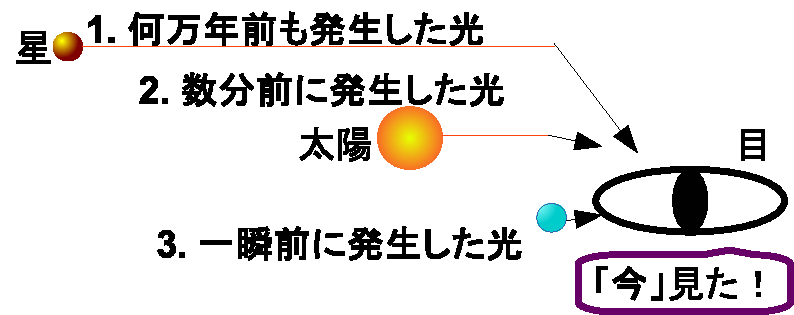
\includegraphics[keepaspectratio, width=7.2cm,height=4.8cm,clip]{star.pdf}
                            \caption{「今」見ている世界}
                            \label{fig:star}
                        \end{center}
                    \end{figure}

                今見ている現象は,いつの現象なのか.光の発生した場所により,
                観測者までの到達時間がばらつくので,観測者が同時にとらえた
                現象でも,実際に発生した時刻は異なるのである.では,
                私は今,いつの世界を見ているのか.「今」という感覚は主観的な感覚であり,
                他人と共有することはできないことは,相対性理論の主張するところであるが,
                相対論を持ち出すまでもなく,「今」という感覚は観測者個人のものでしかない.
                観測者の数だけ異なる「今」がある.

                更に言うなら,目からの視覚情報
                                        \footnote{
                                                視覚情報:目で見た目の前の光景のこと.
                                        }
                を自分が把握するには時間が必要だ.
                脳科学の教えるところによると,「見た」という感覚は,
                目からの情報を脳に伝えて,さらにその情報を脳が処理した結果である.
                ものを「見た」と感じるまでには,目からの情報を脳に伝える時間と,
                その情報を脳が処理して「見た」と感じさせるまでの時間が必要なのだ.
                ということは,今見ていると思っている目の前の光景は過去の光景ということになる.
                つまり,自分自身で感じている「今」も本当の現実世界での今ではなくなってしまう.

                「今」とは,いつのことなのだろうか.

            \end{memo}

            \begin{memo}{空間化された時間}
                時間を計るという行為は,本当に時間を計っているのだろうか.
                フランスの哲学者ベルクソン
                    \footnote{
                        Henri-Louis Bergson(1859--1941,フランス):
                        フランスの哲学者.著書($=$論文)「時間と自由」,「物質と記憶」で有名.
                    }
                は,この問に対して,否定的に答えている.時間を直接的に計れない,というのだ.
                時間を計るには,振り子(振動)にしても,アナログ時計にしても,デジタル時計にしても,
                最終的には,目に見える形で表現されたものを読み取る必要がある.目に見えるということは,
                空間的なものであり,つまり,時間の変化を空間の変化に変換して,時間の変化を捉えている
                のだ.確かに,アナログ時計で時間を計る場合,時間を示す針の位置を見ている.
                時間の変化分を,時計の針の位置の変化分に変換して,計っているのだ.
            \end{memo}

            \begin{memo}{時間の非実在性}
                時間について面白い主張がある.その主張とは,
                「時間という概念に矛盾が存在するので,時間は存在しない」というものだ.イギリスの哲学者,
                マクタガート
                    \footnote{
                        John McTaggart(1866 -- 1925, イギリス):
                        イギリスの哲学者.ラッセル(Bertrand Russell:1872--1970, イギリス)の先生でもある.
                    }
                は,1908年において,時間の非実在性 (The Unreality of Time)を唱えた.
                時間は論理的に存在しないと主張したのだ
                    \footnote{
                        「時間の非実在性(The Unreality of Time)」は,1908年に雑誌Mindで掲載された
                        論文である.もちろん,私はこの論文を読んではいない.以下の本を興味本位で
                        読んだのみである.しかし,この本は,時間の非実在性に関するマクタガートの
                        主張を噛み砕いた,丁寧な説明がなされている.一冊を割いて,この問題を
                        解説している.時間について考えるのであれば,この本を読まないわけにはいかない.
                        ただし,物理学と直接関係したような,重大な問題ではない.
                        私は,こういう考え方もありだな,という程度に捉えている.

                        (参考図書)入不二基義 [著],『時間は存在するか』,講談社現代新書,2002
                    }.
                マクタガートよれば,私達が普段使っている「時間」という概念は,少なくとも2通り存在
                する.一つ目は,時間には,過去$\cdot$現在$\cdot$未来の区別があること
                (この性質をA-系列という).二つ目は,時間の進む向きが過去から未来に向かうこと
                (この性質をB-系列という).この2つの性質を見てみると,B-系列を考えれば,時間に関して
                十分な考察ができると思われる.B-系列が,その内部にA-系列を含んでいるように見えるからだ.
                しかし,マクタガートは時間の性質を考える上ではB-系列だけを考えただけでは,
                時間を十分に捉えることができず,結局,A-系列も前提としなければならないという.
                ところが,このA-系列は,その内部に自己矛盾を含んでおり,とどのつまり,
                時間は存在しないと結論される.

                上記説明は,超概略的な説明でほとんど正確ではない.主張の雰囲気を記述しただけである.
                正確には,脚注に上げた参考図書を読んでもらいたい.
            \end{memo}

            \begin{memo}{時間が逆行しない}
                時間は逆行するか.私が今まで生きてきて,時間が逆行したことは
                ない.もっと正確に言うと,そう感じたことがない.もしかしたら,実際に
                時間は逆行しているが,私達がそう感じていないだけなのかもしれない.
                しかし,それは,私達にとって,時間の逆行したとは言えない.
                自分自身が,時間が逆行していると感じていないと,時間の逆行
                していることを観測したとはいえない.

                私たちは時間の逆行を感じることはできるのだろうか.
                もし,時間逆行を感じ取るには,何か対象となる現象が
                必要である.例えば,コップからこぼれた水がひとりでに
                コップに戻るとか,道路を行き交う車や人々が後ろ向きに
                動いているとかといった,日常で起こりうる現象と反対の
                動きをする現象を見ないといけない.また,その時に時計の針
                    \footnote{
                        デジタル時計であれば,時計に表示される,時間を示す数値.
                    }
                も逆行していることもみないといけない.ここまで見れば,
                時間が逆行しているとみなしてよいだろう.
                本当によいだろうか.周囲が偶然に逆向きに運動していただけ,
                ということは起こり得ないのだろうか.
                今の物理学では,時間の逆行を完全には否定することができない.
                つまり,厳密には,時間が逆行していることの確認は不可能なのである.
                何が足りないのか.時間の定義に何か問題があるのか.
                それとも,何か基本的なことを考え逃しているのか,見逃していいるのか.
                現在の物理学が時間の逆行を許しているにもかかわらず,なぜ,
                私たちは時間の逆行という現象を体験したことがないのだろうか.
                時間の逆行が今までに起こっていないのはなぜか.

                こう考えていても,結論を見いだせそうにない.そこで,発想を
                変えて,時間の逆行を観測したと自分が感じたと仮定してみる.
                この時の,時間逆行の観測者の状況を考えてみよう.
                時間逆行の観測者は,周囲の物体が逆向きに動いているのを
                観測している.見る物体すべてが逆に運動しているのだ.
                では,自分自身はどう観測されるのだろうか.自分自身の
                動きも逆向きに運動していないと,矛盾する.しかし,
                自分の体が逆向きに運動している状況を,観測するという
                状況を想像することは,難しい.少なくとも,それを感じている
                観測者の脳は,時間逆行していてはならない.なぜなら,
                観測者の脳が時間逆行しているとすると,記憶状態が逆向き
                に変化するということであり,記憶が消えて行くということに
                なるからである.記憶が消えてくのにもかかわらず,時間の
                逆行という,新しい現象を記憶することは不可能に思われる.
                こう考えると,時間の逆行を人間が感じ取ることは不可能なのでは
                不可能であることを,強く信じこませられる.時間の逆行を,
                本当に観測することは不可能なのだろうか.
            \end{memo}

%       %======================================================================
%       %  SubSection
%       %======================================================================
        \subsection{長さ}
            私達は「長さ」という概念は直感的に捉えることができる.
            しかし,単に「長い」だとか「短い」だとか
            といっても曖昧である.そこで,長さに基準1[m]をもうけて,
            試料の長さをこれの何倍かで表そう.ここで,
            長さの単位は[m](「メートル」と読む)で表す.
            現在,単位長さ(1[m])長さの定義は,下のように
            なされている.
            \begin{myshadebox}{単位長さ(1[m])の定義}
              1[m]は「真空中で光が 1/299792458 秒間に進む距離」と定義される.
            \end{myshadebox}

            この分数の分母の299792458という数字は光の進む速さに由来する
                \footnote{
                    光速は,$2.99792458\times10^{8}$[m/s] の速度で伝播する.
                    速度の定義は\ref{subsec:Velocity}節を参照.
                }.

            少し唐突な定義だが,今はとりあえずこれを受け止めてもらいたい.
            この定義を理解できるのは,電磁気学で電磁波について学習し終わった頃だろう.
            今すぐに理解できないからといって,あせらないでほしい.

            実は,長さの基準1[m]の定義も,時間の定義と同様に,時代とともに変化する.
            その原因は観測技術の進歩であったり,新しい理論的
            発見が為されることによる.
            従って,このような定義は,いつかは改変されるだろう.
            しかし,長さの基準が変わったからといって,物体の運動法則が変わってしまうかといえば,
            そのようなことは全く起こりえない.単位は人為的に導入するものであり,
            人間が自然を見つめるための1つの道具のようなものに過ぎない.


            現在は,特殊相対性理論が確立しており,この理論によると,
            光の進む速さはどのような速度をもった観測者から見ても一定であるということがわかる.
            これについては特殊相対性理論の部分で確認することだが,
            今はこの事実をそのまま(正しいかどうかは後まわしとして)
            受け入れえておく.このような理由(光の速さが一定であること)から,
            光を基準に取るべきではないかという,
            これまた直感によって規定された定義である.


%       %======================================================================
%       %  SubSection
%       %======================================================================
        \subsection{重さと質量}
            \begin{mycomment}
                「重さ」と「質量」は 万有引力の法則 とニュートンの運動の法則と等価原理を
                考えることによって区別されるものである.つまり,今の段階では,前提となる
                知識が不足していて,その違いを説明することができない.質量とは,運動方程式
                によって,明確に規定される量である.また,重さとは,質量の概念と,
                万有引力の法則によって,定義される量である.しかし,質量や重さのイメージ
                が説明できないわけではない.
                そこで,ここでは,その概要のみだけど,紹介しておく.
            \end{mycomment}

            万有引力の法則によると,質量をもつものは互いに引き合うという性質を
            もっている.例えば,2つのボールが存在すれば,その2つのボールは互いに引き合っている.
            実際には引き合っていないように見えるが,それは力がとても小さいからである.
            実際に引き合うことを説明するために,この2つのボール
            一方を,地球としてみる.当たり前だが,他方のボールは地球に引っ張られて地球に落ちるだろう.
            地球がボールを引っ張っているからである.また,ボールも微力ながら地球を引っ張っている.
            質量が引力を引き起こすのである.

            普段,私達の考えている「重さ」というのは,地球が物体を引っ張る力のことである.
            そこで,この「重さ」というものを基本単位にしようと思ってしまうところだが,
            そうしてしまうとある問題が生じてしまう.
            例えば,
            「地球で自身の体重を測った値」と「別の惑星で自身の体重を測った値」とを比較すると,
            全く異なった値になる.それは,地球と別の惑星の質量の差によっている.
            人間自身は全く同一人物であるから,質量は変化していないはずである.
            一人の人間が色々な惑星にいったとき,その人間を構成する原子や分子
            の量が極端に変化するようなことは理想的にはありえない
                \footnote{
                    理想的にというのは,体調の変化や精神的ストレスなどを
                    無視できるとした場合をいう.
                }.
            それにもかかわらず,
            “重さ”は測る場所によって変化する.従って,重さを基準とすることはできない.
            重さを基準として扱うとなると,いちいち“どこで測ったか”ということを問題に
            しなければならなくなってしまう.

            重さに対して,質量は場所によって変化することない.そこで,重さの変わりに,
            質量を基本単位として
            扱うのである.基準は現在も「キログラム原器」を用いている.単位を [kg] で表現する.
            単位の k は $10^{3}$ を意味する.
            \begin{figure}[hbt]
                \begin{center}
                    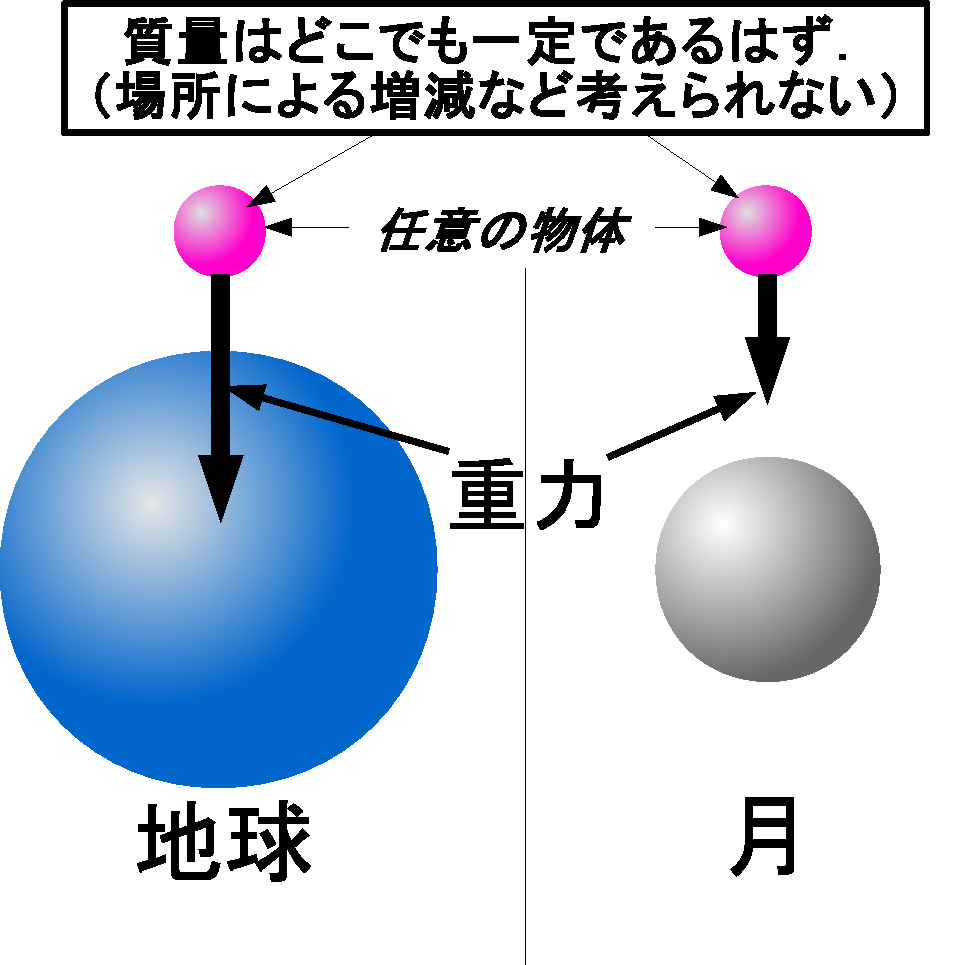
\includegraphics[keepaspectratio, width=6cm,height=6cm,clip]{mass1.pdf}
                    \caption{「質量」と「重さ」の違い}
                    \label{fig:mass1}
                \end{center}
            \end{figure}


            \begin{memo}{定量的な説明}
            \begin{mycomment}
            ここの内容は読み飛ばしてもかまわない.上の説明で,納得がいかなかった場合に読めばよい.
            詳しいことは後で考えることにして,概略を書く.
            \end{mycomment}

            物体 A が物体 B から受ける万有引力 $\bF_{\mathrm{AB}}$ は以下のように表現される.
                    \begin{align}\label{AA}
                        \bF_{\rm{AB}}
                        = -G\frac{m_{\rm{gA}}m_{\rm{gB}}}{{\left| \br_{A}
                        -\br_{B} \right|}^{2}}
                        \frac{\br_{A}-\br_{B}}{\left| \br_{A}
                        -\br_{B} \right|}
                    \end{align}
            ここに,$m_{\rm{gA}}$,$m_{\rm{gB}}$ は2つの物体 A と B のそれぞれの重力質量である.
            $\br_{A}$,$\br_{B}$は,それぞれ$m_{\rm{gA}}$と$m_{\rm{gB}}$の
            位置である.
            「重力質量」とは,万有引力を生じさせる質量のことである.$G$ は万有引力定数
            である.

            式(\ref{AA})で,物体 B を地球であるとすると,物体 A は地球から
                    \begin{align}\label{AAAAA}
                        \bF_{\rm{A-\mbox{地球}}}
                        = -G\frac{m_{\rm{gA}}m_{\rm{g\mbox{地球}}}}{{\left| \br_{A}
                        -\br_{\mbox{地球}} \right|}^{2}}
                        \frac{\br_{A}-\br_{\mbox{地球}}}{\left| \br_{A}
                        -\br_{\mbox{地球}} \right|}
                    \end{align}
            の力を受ける.
            ここで,添え字の「地球」は地球に対する質量や位置を表している.
            地球の質量 $m_{\rm{g\mbox{地球}}}$ と物体 A の位置 $\br_{A}$ は
            一定であるから,
                    \begin{align}\label{AAAAAA}
                        \textit{\textbf{g}}_{\mbox{地球}}
                        := -G\frac{m_{\rm{g\mbox{地球}}}}{{\left| \br_{A}
                        -\br_{\mbox{地球}} \right|}^{2}}
                        \frac{\br_{A}-\br_{\mbox{地球}}}{\left| \br_{A}
                        -\br_{\mbox{地球}} \right|}
                    \end{align}
            と置けば,式(\ref{AAAAA})は
                    \begin{align}\label{AAAAAAA}
                        m_{\rm{gA}}\textit{\textbf{g}}_{\mbox{地球}}=\bF_{\rm{A-\mbox{地球}}}
                    \end{align}
            と書ける.$\textit{\textbf{g}}_{\mbox{地球}}$ は \textbf{地球の重力加速度}とよばれる.

            重さとは,式(\ref{AAAAAAA})の右辺の $\bF_{\rm{A-\mbox{地球}}}$ のことであり,
            これは地球に引っ張られる力を意味している.対して,質量とは,式(\ref{AAAAAAA})の左辺の $m_{\rm{gA}}$ の
            ことである.重さが測る場所で変化するというのは,式(\ref{AAAAAA})の質量部分 $m_{\rm{g\mbox{地球}}}$ が
            惑星ごとに異なるためである.従って,重さが変化するのは $\textit{\textbf{g}}_{\mbox{地球}}$ が変化することが原因であって,
            $m_{\rm{g\mbox{地球}}}$ は何ら関係がない.質量とは,重さに含まれる力を取り除いた概念である.以上が
            重さと質量の違いである.
            \end{memo}

            \begin{memo}{お肉の重さ}
            質量と重さのもっと身近な例をあげよう.例えば,那覇で1[kg]の牛肉を
            買ったとしよう.那覇の重力加速度を9.80[m/s${}^{2}$]とすると,
                \begin{equation*}
                    \mbox{重さ} W = \mbox{質量} m_{\mathrm{i}} \times \mbox{重力加速度} \textit{\textbf{g}}
                \end{equation*}
            だから,$W=$1[kg]$\times$9.80[m/s${}^{2}$]$=$9.80[kgf] である.ここに,[kgf]は
            重さの単位で,“kilogram-force(キログラム・フォース)”という
                \footnote{
                    [kgw] と書いて,“kilogram-weight(キログラムウェイト)”ということもある.この場合は
                    日本語では「キログラム重(---ジュウ)」とよくいわれる.
                }.
            この9.80[kgf]の牛肉を,札幌にもっていくとどうなるだろうか.
            札幌の重力加速度は約9.79[m/s${}^{2}$]だから,
            つまり札幌でのこの牛肉の重さは$W=$1[kg]$\times$9.79[m/s${}^{2}$]$=$9.79[kgf] である.
            この那覇からもってきた9.80[kgf]の牛肉は
            札幌では9.79[kgf]になってしまうのである.
            別に質量が減ったのではない.那覇でも札幌でも1[kg]の牛肉である.それにもかかわらず,
            重さが0.01[kgf],つまり10[gf]も変わってしまうのである.
            実際はこのようなことが起こらないように,
            札幌と那覇でのはかりは重力加速度の違いを考慮して作られている.
            重さと質量の違いを身近に感じるのではないだろうか.
            \end{memo}


            \begin{memo}{質量は「何」からできているか}
            力学を勉強するときには,「質量」という概念は有無を言わさずに,受け入れさせられる
            はずである.しかし,この質量とはいったい何かを考えたくもなるものである.
            実際,物理学者はこの問題を考え,原子というものを発見したし,さらには,
            電子や陽子,中性子を発見している.現在では,さらに素粒子,クォークと
            どんどん詳細なことが見つかっている.では,質量は素粒子から生じているのか.
            いや,実はそうではない.素粒子は質量をもたない.では,質量はどこから生じているのか.
            この問題は「素粒子物理学」が解決してくれるものだと思う.大統一理論だとか,超ひも理論
            だとかで有名であるが,まだ完全には説明しきれていないようである
                \footnote{
                    私は啓蒙書を読んだ程度の知識なので,質量が現在どのように説明され,
                    その説明がどのように不完全なのかを握していない.
                    この理解についても,生涯の目標にしたい.
                    ただ,とても難しい数学的演算を必要とするみたいなので,これは,難しいかも...
                }.
            そんなわけで,今は質量の発生源を探ることはせず,まずは質量ありきの理論を学習しよう.

            「質量」はニュートン力学では当たり前のように使われる概念であり,物理学の基本中の基本であるが,
            その詳細は分かっていない.油断すると,質量というものは存在して当たり前だと思い,
            見過ごしてしまうかもしれない.頭の片隅に,この問題を記憶しておこう.
            \end{memo}

%       %======================================================================
%       %  SubSection
%       %======================================================================
        \subsection{基本単位のまとめ}
            以上で,基本単位の説明が終わった.
            この他にも電磁気学では電流の単位[A](アンペア)があるが,
            力学では電流という概念は扱わないのでここでは省略する.
            電磁気学の部分で電流の単位を確認することにしよう.
            さて,力学の基本単位はSI系で[s],[m],[kg]である.
            それぞれ時間,長さ,質量の単位である.
            単位の定義についてもう一度確認しておきたい.

            まず,時間の基本単位1[s]を定義した.それは「$^{133}${\rm Cs} 原子が 9192631770 回振動する時間」を1[s]とする
            というものであった.次に,この時間の単位を踏まえたうで,長さの基本単位1[m]を定義した.1[m]の定義は,
            「真空中で光が 1/299792458 秒間に進む距離」であった.
            これは光速を基とした定義である.
            そして,この2つの基本単位とは独立して,質量の基本単位1[kg]を定義した.
            といっても,質量の基本単位はキログラム原器である.
            キログラム原器の重さ1[kgf]を基にしている.


            \begin{memo}{各基本単位の関係}
            ニュートンの運動方程式は $ma=F$ である.ここに,$m$ は質量,$a$ 加速度,$F$ は力である.
            高校でも学習したように,質量 $m$ の単位は[kg],加速度 $a$ の単位は[m/s${}^{2}$]である.
            従って,力 $F$ の単位は[kg$\cdot$m/s${}^{2}$]である.力の単位としては[N](ニュートン)を
            用いることが多く,従って,
                \begin{equation*}
                    1[\mathrm{N}]=1[\mathrm{kg}\cdot\mathrm{m}/\mathrm{s}^{2}]
                \end{equation*}
            である.

            先走って書いてしまえば,電流の基本単位[A](アンペア)の定義はこの1[N]を元にして定義されている.
            どのように定義するかは電磁気学の部分で確認しよう.アンペアの定義が
            確認できたとして,物理学におけるSI系の基本単位の構成図を書いておくと,
            明瞭になると思う
                \footnote{
                    電子情報通信レクチャーシリーズ B-13,電子情報通信学会 編,
                    岩崎 俊 [著],『電磁気計測』,page 23,2006から.
                }.
                \begin{figure}[hbt]
                    \begin{center}
                        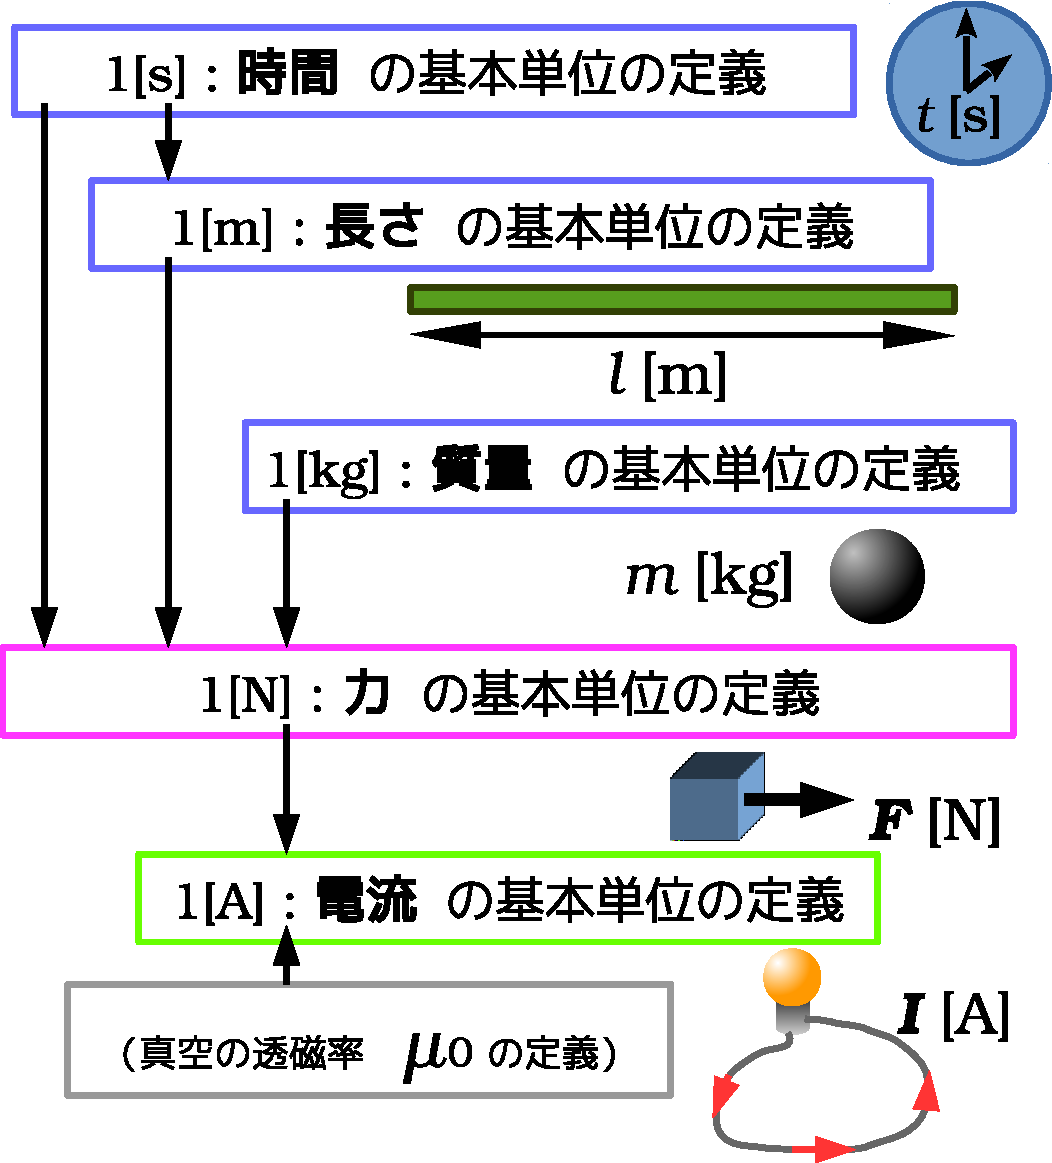
\includegraphics[keepaspectratio, width=7cm,height=8.42cm,clip]{tanni1.pdf}
                        \caption{単位の構成}
                        \label{fig:tanni1}
                    \end{center}
                \end{figure}

            最初に,原子の出す光の振動回数から,1[s]が定義される.
            そして,1[m]を光が1[s]で進む距離の1/$c$ ($c$ は光速の数値)と定義される.
            また,質量は,これらとは独立に,キログラム原器を基準に1[kg]が定義される.
            ちなみに,この1[s],1[m],1[kg]から力の単位[N](=[kg$\cdot$m/s${}^{2}$)が
            定義され,この1[N]を用いて,電流1[A]が定義される.電流の単位については
            電磁気学の項目を参照のこと.
            \end{memo}

%   %==========================================================================
%   %  Section
%   %==========================================================================
    \section{物理学における,数学の扱い方}
%       %======================================================================
%       %  SubSection
%       %======================================================================
        \subsection{道具としての数学}
            先に,物理学では数学を道具として扱うと説明した.道具として扱うとは,
            数学的厳密性を適宜無視して,数式を扱うということである.物理学の目的
            は自然現象を数式で表現することであり,重要なのは数式ではなく自然現象
            である.だから,物理学の教科書を読んでいて,数式が出てきた場合に,注
            意が必要なのである.

            数学を学習する上で大切なことのひとつに,厳密な証明の理解がある.だけ
            ど,数学を厳密に扱うとは,物理学ではあまり行わない.むしろ,厳密性を
            無視してしまっていることが多い
                \footnote{
                    例えば,テイラー(Sir Brook Taylor, 1685--1731, イギリス)展開
                    の高次の項は無視するということがある.
                }.

            物理学における数学は,あくまで道具なので,そんなに厳密に考える必要は
            ない.大切なのは,そのイメージできることである.研究者になるのでない
            限り,数学的厳密性に敏感になるよりも,数学を図形的にイメージできるよ
            うになることの方が大事である.言うまでもなく,私は研究者を目指してい
            るわけではないので,このノートでも数学的厳密性は全く気にしていない.
            このノートでは,数学を直感的に扱える程度で十分である.


%       %======================================================================
%       %  SubSection
%       %======================================================================
        \subsection{物理学の考え方}
            数学の命題や定義は絶対に不変である.後になって「間違いでした」なんて
            ことは起こらない.しかし,物理では間違いは起こる.そのたびに,修正が
            なされる.物理は実験や経験を基にしているからである.物理学ではある問
            題に対して,その原因をいろいろ仮説を立てて,実験的に仮説の正しさを確
            かめる.ここに人間の直感が介入してくる.この「人間の直感」こそが,数
            学と物理の大きな違いである.

            物理学は,感覚的なひらめきを基に構成される.だから,このひらめきが正
            しいかどうかを確認すべきだ.そのために,ひらめきを数式で表現
            して,実際に実験して検証する必要がある.物理学は,ひらめきとイメージ
            に重点が置かれているといってもよい.

            数学では考えられないことだろう.数学でも,問題を解くときにはひらめき
            はとても重要だ.そうなのだけど,物理学との違いはその検証の方法であ
            る.数学での検証は,数と論理のみで行う.そこには,実験や経験といった,
            人間の直感は含まれない.数学ではこの検証のことを「証明する」という.
            証明は数と論理で構成されいて,一度正しさが確認されれば
                \footnote{
                    (証明の)正しさの確認:論理に間違いがないことを確認すること.
                }
            後になって,間違いでしたということはない.数学に対して,物理学では,
            実験を行って,その検証を行う.実証するしかないのである.物理学では,
            証明はありえない.

            この実験が物理学の醍醐味なのだろう.自然を肌で感じ,数式で表現しさま
            ざまな予測を立てて,検証を行う.これが楽しいから,物理学があるのだ.


%       %======================================================================
%       %  SubSection
%       %======================================================================
        \subsection{物理学の数式の解釈}
            物理法則を表す数式において,等号は「\textbf{近似的に}等しい」という意味で使われる.

            数学における等号は,その右辺と左辺が全く同等であるという意味であ
            る,しかし物理では,例えば法則を数式で書き表すときに,右辺と左辺
            は本来は別々な概念であるのに,それらが等しいと書き表す.このよう
            なときに使われる等号は,“近似的”というような意味での等号である
            と考えるべきだ.この近似的という言葉も正確ではないが.なんという
            か,物理学独特の等号の使い方である.この原因は,物理学では,数学
            のような理論的厳密性よりも,\textbf{実験結果,経験が重要視される} と
            いうところにある.というのも,実験で得られる数値の桁は有限の桁で
            あり,それはもう既に近似である.だから,実験で得られる各法則も近
            似的であるし,物理の理論はこの近似の上で成立している.

            また,等号は定義するときに用いられることもある.

            もちろん,数学的な式変形のときの等号は,
            数学における等号の意味と同じである.
            これは,\textbf{恒等式} といわれる.

            \begin{memo}{恒等式}
                \textbf{恒等式} とは,変数 $x$ にどのような数を代入しても成立する
                式のことである.例えば,因数分解の公式
                    \begin{align}
                        {(x+y)}^{2}=x^{2} + 2xy + y^{2}
                    \end{align}
                がある.この式の $x$,$y$ にどのような数を代入しても,“恒に”成
                立する式である.
            \end{memo}

            \begin{memo}{方程式}
                式には,恒等式の他にも,\textbf{方程式} もある.方程式とは,例えば,
                変数 $x$ がある特別な数のときのみに成立する式のことである.その例
                として,以下の方程式を挙げよう.
                    \begin{align}
                        x^{2} - 2x + 1 = 0
                    \end{align}
                この式は,$x=1$ の場合のみにしか成立しない.このような特定の数値の
                みで成立する式が,方程式である.
            \end{memo}


%   %==========================================================================
%   %  Section
%   %==========================================================================
    \section{対称性 --- 物理学の基本要請 ---}
    \begin{mycomment}
        ここで,物理学の最も基礎となる考え方である,\textbf{対称性} について
        説明する.
        物理学には,その思想の基礎に,\textbf{対称性} という考え方を持っている.
        対称性とは,その名の通り,「どちらを見ても同じ」ということである.
        対称性という言葉は,実は,中学生の頃から使用している.
        例えば,点対称な図形は180${}^{\circ}$ 回転しても形を変えないという性質
        を持っている.また線対称な図形とは,左右あるいは上下で鏡を写したような
        形のことである.
        物理学で言う所の対称性は,点対称や線対称と同じような意味である.
        ただ違う点は,対象が図形ではなく,空間と時間に関する法則の性質である
        ことだけである.
        空間や時間の対称性とはとういうことかを,この節で説明していく.
    \end{mycomment}

%       %======================================================================
%       %  SubSection
%       %======================================================================
        \subsection{空間の対称性}
            \begin{mycomment}
                空間の対称性には2種類あり,次の通りである.
                    \begin{itemize}
                        \item 並進対称性
                        \item 回転対称性
                    \end{itemize}
                これらについて,以下で説明する.
            \end{mycomment}
%           %==================================================================
%           %  SubsubSection
%           %==================================================================
            \subsubsection{並進対称性}
                空間の並進対称性とは,どの方向に並行移動しようが,物理法則は
                全く変化しないということである.

                具体例で説明しよう.ある場所Aで実験していて,ある結果を得たとし
                よう.この実験結果は間違いがないものと,裏付けられたとする.こ
                の実験を別の場所Bで,全く同様の条件と方法で実験を行ったとき,
                実験結果はどうなるだろうか.全く同じ結果
                    \footnote{
                        実験誤差は当然考慮した上で.
                    }
                になるはずである.そうならなくては,その実験は正しいとは言えない.
                “どんな場所で,実験しても,実験条件と方法が同じであれば,同一の結果を得る”
                という考え方が,\textbf{空間の並進対称性} である.空間の並進対称性
                を信じているからこそ,正しい実験とその結果を受け入れることができるのである.
                ただし,並進対称性は,並進と言っているからには,実験している方向に
                関しては,していない.つまり,“同一の向きを向いて”という仮定が
                含まれているのである.

                もう一度言おう.空間の並進対称性は,場所Aで実験しても,
                場所Aから平行移動した場所Bでも,条件と方法が同じであれば,
                得られる結果も同じになるということを保証する.

                つまり,「どこで実験しても得られる結果は同じ」ということである.
                言い換えれば,\textbf{物理法則は場所により不変である}と言える.
                    \begin{myshadebox}{空間の並進対称性}
                        \textbf{空間の並進対称性} は,物理法則は場所によって不変であることを
                        主張するものである.
                    \end{myshadebox}

                    \begin{figure}[hbt]
                        \begin{center}
                            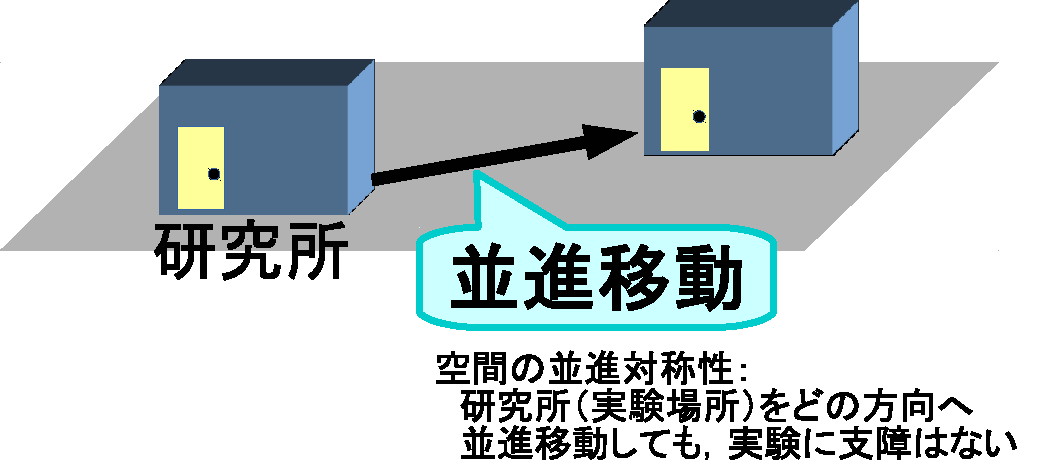
\includegraphics[keepaspectratio, width=7cm,height=3.23cm,clip]{Synmmetry_SpaceP.pdf}
                            \caption{研究所の並進移動}
                            \label{fig:Synmmetry_SpaceP}
                        \end{center}
                    \end{figure}


%           %==================================================================
%           %  SubsubSection
%           %==================================================================
            \subsubsection{回転対称性}
                並進対称性では,並進移動しても物理法則に何ら変化がないということが
                保証される.これに対して,回転対称性は,その名の通り,回転しても
                物理法則が変わらないことを保証している.ある向きで実験を行った
                とし,その後,同じ場所で別の向きで実験しても,向きを変える前と
                実験結果は同一になるということである.

                つまり,
                \textbf{空間の回転対称性} は,
                ある場所において,ある向きで実験する場合と,その場所で別の向きで
                実験する場合とで,同じ結果を得ることを保証する.

                つまり,「どの向きで実験しても,得られる結果は同じ」ということである.
                言い換えると,\textbf{物理法則は向きに対して不変である}と言える.
                    \begin{myshadebox}{空間の回転対称性}
                        \textbf{空間の回転対称性} は,物理法則が向きに対して不変である
                        ことを主張するものである.
                    \end{myshadebox}

                    \begin{figure}[hbt]
                        \begin{center}
                            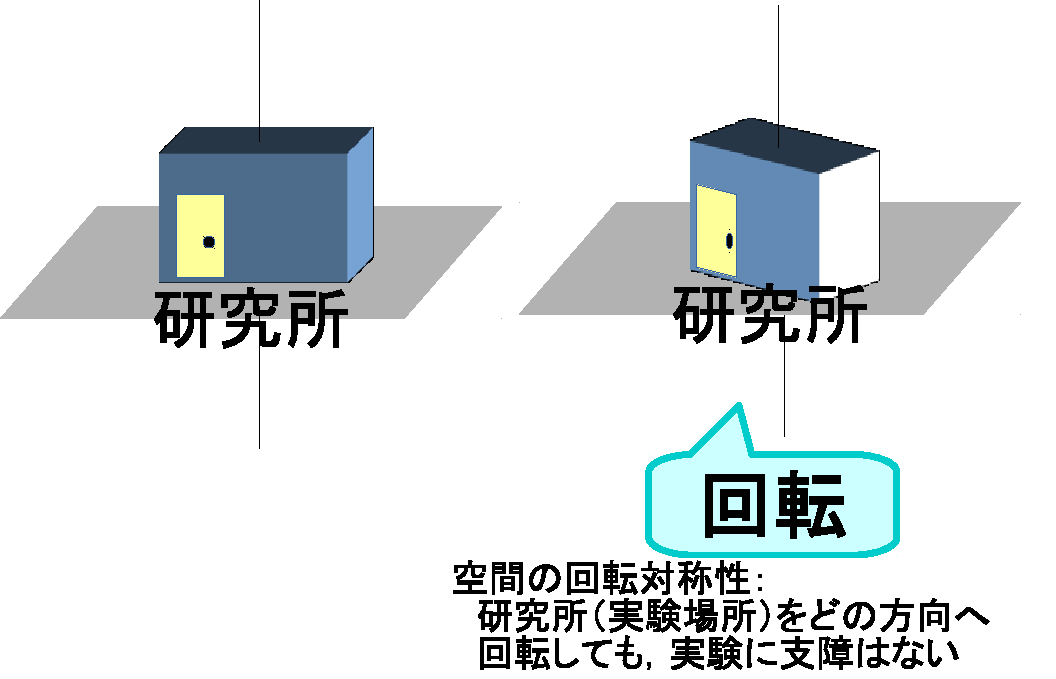
\includegraphics[keepaspectratio, width=7cm,height=4.6cm,clip]{Synmmetry_SpaceR.pdf}
                            \caption{研究所の回転}
                            \label{fig:Synmmetry_SpaceR}
                        \end{center}
                    \end{figure}


%       %======================================================================
%       %  SubSection
%       %======================================================================
        \subsection{時間の対称性}
            時間の対称性が意味するところは,とても単純で,
            物理法則が時間に対して不変であることを主張するものである.
            要するに,いつ実験しようが実験結果は変わらないということ
                \footnote{
                    もちろん,条件,方法は同じである必要がある.
                }.
            朝に実験しようが,夜中に実験しようが,実験結果は全く同じ.
            朝の実験の方が良い結果を生むということは決して無い.
                    \begin{myshadebox}{時間対称性}
                        \textbf{時間の対称性} は,物理法則が時間に対して不変である
                        ことを主張するものである.
                    \end{myshadebox}


%       %======================================================================
%       %  SubSection
%       %======================================================================
        \subsection{対称性 --- まとめ ---}
            \textbf{対称性} という専門用語を使うと,いかにも難しい概念だと思われる
            が,その意味はとても単純であり,私たちには暗黙の了解として体に染み付い
            ているものである.対称性のおかげで,研究所を建てる場合に,場所や向きや
            時代を考えることは必要がなくなる.いや,そもそも,物理法則は場所や向き,
            時間に対して不変でなければならないという要請がなされているものである,
            といった方が正確だ.

            つまり,物理法則というからには,対称性を備えていなければならない
            のである.物理法則は,場所にかかわらず,向きにかかわらず,時間(時代)
            にかかわらず,不変性を保つものである.
                    \begin{myshadebox}{対称性}
                        \textbf{対称性} は,物理法則に要請される性質の1つである.
                        物理法則は,場所や向き,時間にかかわらず不変でなければならない,
                        という要請である.対称性により,物理法則が不変であることを
                        保証するのである.
                    \end{myshadebox}


%       %======================================================================
%       %  SubSection
%       %======================================================================
        \subsection{対称性と保存則(ネーターの定理)}
            対称性からとても大切な性質が導かれる.詳細は,解析力学を
            学習するときに確認することだが,ここでは簡単に紹介しておこう.

            唐突で申し訳ないが,下表(\ref{tab:Synmmetry_and_Conservation})をみて
            欲しい.この表を見ながら,以下の説明を読んでもらうと,幾らかは
            わかりやすいと思う.
            \begin{table}[hbt]
                \label{tab:Synmmetry_and_Conservation}
                \caption{対称性と保存則の関係}
                \begin{center}
                    \begin{tabular}{l|l}
                        \multicolumn{1}{c|}{対称性} & \multicolumn{1}{c}{保存則} \\
                        \hline\hline
                        時間の対称性 & エネルギー保存の法則 \\
                        \hline
                        空間の並進対称性 & 運動量保存の法則 \\
                        \hline
                        空間の回転対称性 & 角運動量保存の法則 \\
                        \hline
                         ゲージ対称性 & 電荷保存の法則 \\
                    \end{tabular}
                \end{center}
            \end{table}

            物理学を学習していくと,場所や向きや時間に影響されない法則を
            見つけることができる.これは \textbf{保存則} と言われる.
            例えば,中学生の頃からおなじみの,力学的エネルギー保存の法則が
            ある.これも,保存則の1つである.更にこれを一般化して,
            単に,\textbf{エネルギー保存の法則} とされるが,このエネルギー保存則
            は時間の対称性から数学的に導かれるのである
                \footnote{
                    “導けてしまう”と言ったほうが,実際的かもしれない.
                    感覚は人それぞれだけども$\cdots$.
                }.
            つまり,数学の定理
            である \textbf{ネーターの定理}に時間の対称性を照らし合わせると,
            エネルギーがいつでも一定値をとる
                \footnote{
                    いつでも一定値をとることを,\textbf{保存する} という.
                    詳細は後述する.
                }
            ことが結論されるのである.

            同様に,空間の並進対称性からは,\textbf{運動量保存の法則} が得られる.
            また,空間の回転対称性からは,\textbf{角運動量保存の法則} が得られる.
            また,ゲージ対称性からは,\textbf{電荷保存の法則} が導かれる.
            ネーターの定理の具体的な意味と保存則に関する詳細は,後に改めて考えることとし,
            ここでは紹介程度にとどめる.
